\documentclass[11pt]{article}
\usepackage[letterpaper,margin=0.88in]{geometry}
\usepackage[T1]{fontenc}
\usepackage{lmodern,microtype}
\usepackage{amsmath,amssymb,amsthm,booktabs,array,graphicx}
\usepackage[dvipsnames]{xcolor}
\usepackage[colorlinks=true,linkcolor=MidnightBlue,urlcolor=MidnightBlue,citecolor=MidnightBlue]{hyperref}
\usepackage{enumitem}
\setlist{nosep,leftmargin=*}
\setlength{\parskip}{4pt}
\setlength{\parindent}{0pt}
\setlength{\emergencystretch}{2em}
\clubpenalty=10000
\widowpenalty=10000
\newtheorem{proposition}{Proposition}
\newtheorem{corollary}[proposition]{Corollary}
\newcommand{\Prb}{\mathbb P}
\newcommand{\E}{\mathbb E}
\newcommand{\ind}{\mathbf 1}
\title{Probability Laws for No-Guess\, Minesweeper Generation}
\author{Minesweeper Exploration}
\date{October 26, 2026}
\begin{document}
\maketitle
\begin{abstract}
No-guess generation changes the distribution of mine layouts. The change is not adequately described as placing mines ``less randomly'': it depends on the proposal distribution, the protected starting region, the certifying solver, and whether failed layouts are rejected or repaired. We derive the conditional law of rejection generation, distinguish sequential logical completion from static uniqueness, and show when protecting a zero opening accelerates generation without changing the accepted distribution. Exact enumeration of all 560 three-mine layouts on a $4\times4$ board separates the effects of starting location and solver strength. For a protected corner opening, a direct-rule solver accepts 44 of 220 layouts, the implemented subset solver accepts 165, and an exact logical solver accepts 181. Conditioning on subset-solvability changes the eligible-cell mine probabilities from a common 25\% to values between 20.61\% and 30.30\%. A reproducible 10,000-output rejection experiment verifies the corresponding marginal and geometric predictions. These are results for declared models and an inspectable local implementation, not an inference about a proprietary website's generator.
\end{abstract}

\section{A fixed-mine baseline and a precise no-guess event}

Let $V$ be a board with $N$ cells, $m$ the fixed mine count, and $s$ the chosen first cell. A layout is a subset $L\subseteq V$ with $|L|=m$. Write $\mathcal N(s)$ for its neighboring cells under the usual eight-neighbor rule. A protected set $E_s$ distinguishes two common first-click contracts:
\[
 E_s^{\rm safe}=\{s\},\qquad
 E_s^{\rm zero}=\{s\}\cup\mathcal N(s).
\]
The ideal baseline is uniform over eligible layouts,
\begin{equation}
 \Omega_{E_s}=\{L\subseteq V\setminus E_s:|L|=m\},\qquad
 P_0(L\mid s,E_s)=\frac{\ind\{L\in\Omega_{E_s}\}}{\binom{N-|E_s|}{m}}.
 \label{eq:baseline}
\end{equation}
This requires $m\le N-|E_s|$; otherwise the requested protection is infeasible. A fallback that protects only $s$ is a different proposal law and must be identified as such.

Uniformity over layouts does not mean independent mine indicators. Put $n=N-|E_s|$ and $\rho=m/n$. For distinct eligible cells $i,j$, with $n>1$,
\begin{equation}
 \Prb(i\in L)=\rho,\quad
 \Prb(i,j\in L)=\frac{m(m-1)}{n(n-1)},\quad
 \operatorname{Cov}(\ind_{i\in L},\ind_{j\in L})=-\frac{\rho(1-\rho)}{n-1}.
 \label{eq:cov}
\end{equation}
The negative dependence enforces the fixed total. All eligible cells have the same marginal before further selection, despite corners and interior cells having different geometric roles. Protected cells have probability zero.

After an opening, a visible state $O$ consists of revealed safe cells and their clues. Let $\mathcal C(O)$ be the layouts consistent with those observations, the total mine count, and the declared protection. An \emph{exact forced safe cell} is safe in every member of $\mathcal C(O)$. A sound solver $S$ may reveal only cells it proves safe from this information; it may also derive mines. The actual layout supplies new clues only after a justified reveal. Automatic zero flooding is included.

Define the sequential acceptance event
\begin{equation}
 A_S(L,s)=\{S\text{ reveals every safe cell of }L\text{ after the prescribed start }s\}.
 \label{eq:event}
\end{equation}
The solver's rules, resource bounds, and move-selection policy are part of this definition. For the exact solver used below, all currently forced safe cells are revealed at each step; a stall means none exists. A bounded solver can reject a board that stronger sound reasoning completes. Its rejection is therefore not evidence that guessing is mathematically necessary.

Static uniqueness is a different property. If $|\mathcal C(O)|=1$, exact inference identifies every hidden cell, but a limited solver need not find that proof. Conversely, sequential no-guess completion can begin with many consistent layouts: new safe clues disambiguate them. Our enumeration includes a subset-solvable opening with two initial consistent layouts, and an exactly solvable opening with 28 initial consistent layouts that the subset solver cannot advance. Neither an ordinary game's fixed hidden layout nor a completed solution establishes initial clue uniqueness.

\section{The distribution produced by rejection}

Fix $s,E_s,S$. Let proposals $L_1,L_2,\ldots$ be independent draws from $P_0$, and accept the first satisfying $A_S$. Put $p=P_0(A_S)$.

\begin{proposition}[Conditional output law]
If $p>0$, the first accepted layout has distribution
\begin{equation}
 Q_S(L\mid s)=\frac{P_0(L\mid s,E_s)\ind\{A_S(L,s)\}}{p}.
 \label{eq:rejection}
\end{equation}
For the uniform baseline, this is uniform over the \emph{solver-accepted subset}, not over all fixed-mine layouts or necessarily all exactly solvable layouts.
\end{proposition}
\begin{proof}
For a particular accepted layout $L$, its probability of being returned on proposal $t$ is $(1-p)^{t-1}P_0(L)$. Summing over $t\ge1$ gives $P_0(L)/p$. Rejected layouts have zero output probability.
\end{proof}

The number of proposals $T$ is geometric:
\begin{equation}
 \Prb(T=t)=(1-p)^{t-1}p,\qquad \E T=\frac1p,\qquad
 \Prb(T>K)=(1-p)^K.
 \label{eq:geometric}
\end{equation}
A fixed cap $K$ creates a failure outcome, but, conditional on returning a board, leaves the law in \eqref{eq:rejection} unchanged. Indeed, summing only to $K$ multiplies every accepted layout's probability by the same factor $[1-(1-p)^K]/p$. The expected number of proposals actually executed is
\begin{equation}
 \E\min(T,K)=\sum_{t=1}^K\Prb(T\ge t)=\frac{1-(1-p)^K}{p}.
 \label{eq:cap}
\end{equation}
For $p=0$, no valid output exists under that solver and proposal; every capped run uses $K$ proposals. An attempt cap is not a wall-clock cap: solver costs can vary by board. A time budget, adaptive proposal changes, or returning the ``best failed'' candidate does not inherit the conditional-law result without a new argument.

The mine marginal after selection follows directly:
\begin{equation}
 Q_S(i\in L)=\frac{P_0(i\in L, A_S)}{P_0(A_S)}.
 \label{eq:marginal}
\end{equation}
Cells may cease to be exchangeable because the acceptance event depends on their geometry relative to the start and the rest of the board. Uniform probabilities for whole accepted layouts are entirely compatible with unequal probabilities for individual cells.

\section{Why a safe-only no-guess start often opens a zero}

Suppose the first reveal shows a positive clue $k$, so zero flooding has not occurred. Let $d=|\mathcal N(s)|$ and $q=N-1-d>0$. With no other observations, the compatible layouts distribute $k$ mines among the $d$ neighbors and $m-k$ among the $q$ remaining cells. There are
\begin{equation}
 \binom d k\binom q{m-k}
 \label{eq:firstcount}
\end{equation}
such layouts under safe-only protection. Hence an individual neighbor has mine probability $k/d$, and an individual non-neighbor has probability $(m-k)/q$. If both fractions are strictly between zero and one, no hidden cell is forced safe or forced mined. At a saturated endpoint a group is known; that must not be mistaken for the generic case.

\begin{proposition}[A sufficient condition for a zero start]
If $m>d$ and $m<q$, a positive first clue supplies no forced safe next reveal under clue-only exact reasoning. Therefore $A_S(L,s)$ implies a zero first clue for every sound solver using only that information.
\end{proposition}
\begin{proof}
For $1\le k<d$, both groups have a strictly positive, non-unit mine fraction. For $k=d$, all neighbors are mines, but $0<m-d<q$, so every non-neighbor remains ambiguous. Flagging the already implied neighboring mines adds no clue and produces no new safe reveal. In either case the safe cells required to finish cannot all be revealed without a guess.
\end{proof}

The conditions hold at every starting cell on the conventional Beginner $(81,10)$, Intermediate $(256,40)$, and Expert $(480,99)$ boards. They need not hold for unusual tiny or dense boards. For example, on a $4\times4$ board with three mines, a corner clue of three locates all mines and proves every non-neighbor safe. Our exact enumeration includes this positive-start no-guess board. At an interior start, a clue equal to the total mine count can similarly prove the outside region safe. ``No guess always means a zero first clue'' is therefore too broad.

For a safe first cell, let $Z$ denote a zero clue. Under the ideal law, for $z>0$,
\begin{equation}
 z=P_{\rm safe}(Z)=\frac{\binom{N-1-d}{m}}{\binom{N-1}{m}},\qquad
 P_{\rm zero}=P_{\rm safe}(\,\cdot\mid Z).
 \label{eq:zero}
\end{equation}
\begin{corollary}[A more efficient equivalent proposal]
If $A_S\subseteq Z$ and $P_{\rm safe}(A_S)>0$, the same solver protocol gives
\begin{equation}
 p_{\rm safe}=z\,p_{\rm zero},\qquad
 P_{\rm safe}(\,\cdot\mid A_S)=P_{\rm zero}(\,\cdot\mid A_S).
 \label{eq:equivalent}
\end{equation}
Thus zero-protected proposals reduce the expected proposal count by a factor $1/z$ without changing the accepted distribution.
\end{corollary}
\begin{proof}
Positivity and $A_S\subseteq Z$ imply $z>0$ and $P_{\rm safe}(A_S)=zP_{\rm safe}(A_S\mid Z)$. Conditioning either baseline further on $A_S$ cancels $z$.
\end{proof}

For a corner, $z$ is 0.66626, 0.59805, and 0.49846 at the three standard difficulties. The ideal reductions are consequently factors of 1.501, 1.672, and 2.006. These are proposal-count factors, not measured wall-clock speedups. They also explain why observing zero openings from a safe-only NG generator does not establish that its implementation explicitly protected the whole neighborhood.

\section{Starting cells, stochastic acceptance, and repaired boards}

Starting-location policy matters. Suppose a start is sampled with probability $w_s$, and let $p_s=P_0(A_S\mid s)$. If $s$ is sampled once and held fixed while layouts are rejected until success, with $p_s>0$ for every selected start, the joint output law is
\begin{equation}
 Q_{\rm held}(L,s)=w_s\frac{P_0(L\mid s)\ind\{A_S(L,s)\}}{p_s}.
 \label{eq:held}
\end{equation}
The output start probabilities remain $w_s$. If the pair $(L,s)$ is resampled after every rejection instead, then
\begin{equation}
 Q_{\rm pair}(L,s)=\frac{w_sP_0(L\mid s)\ind\{A_S(L,s)\}}{\sum_u w_up_u},\qquad
 Q_{\rm pair}(s)=\frac{w_sp_s}{\sum_u w_up_u}.
 \label{eq:pair}
\end{equation}
Easier starts become more common among outputs. With a fixed per-start cap and failure runs discarded, held-start weights instead become proportional to $w_s[1-(1-p_s)^K]$. Reporting only successful boards can therefore change the observed mix even when each attempt obeys its own baseline.

For a randomized certifier, let $a(L,s)\in[0,1]$ be its acceptance probability, including any independent random choices or random limits. Independent repeated proposals and certifier randomness give
\begin{equation}
 Q(L\mid s)=\frac{P_0(L\mid s)a(L,s)}{\sum_{L'}P_0(L'\mid s)a(L',s)}.
 \label{eq:soft}
\end{equation}
A board accepted with probability one receives twice the weight of an otherwise equally likely board accepted with probability one half. Uniformity on all potentially accepted boards is no longer assured.

Repair and constructive generation require another model. If a proposal $L$ is transformed by a randomized kernel $K(L,L')$, the output law is
\begin{equation}
 Q(L')=\sum_L P_0(L)K(L,L').
 \label{eq:kernel}
\end{equation}
Many input layouts may map to the same output, and the transition weights need not balance. Moving mines to remove ambiguities does not automatically sample uniformly from solvable boards. After a repair, the \emph{final} layout must be re-certified from the promised start: a proof made using clues that existed before modification is not a certificate for the changed board. Similar caution applies to first-click mine relocation. A particular relocation rule can preserve a desired distribution, but that requires proof for that rule; it is not a universal consequence of moving the clicked mine elsewhere.

Inspectable implementations demonstrate that ``NG'' names different mechanisms. The examined Simon Tatham Mines source starts with a protected opening, allows mine perturbations when deduction stalls, and repeats a solve until no perturbation is needed~\cite{tatham}. The examined JSMinesweeper generator starts with a zero-mode board and processes solver-provided fillers through its repair routine~\cite{js-source}; its documentation separately distinguishes a safe first click from an opening and warns that a replay may cease to be no-guess from another start~\cite{js-doc}. These source-specific observations do not establish a distribution for Minesweeper Online, whose help describes the NG promise rather than a complete sampling algorithm~\cite{wom}.

\section{Exact enumeration and a sampling check}

We enumerate every one of the $\binom{16}{3}=560$ layouts on a $4\times4$ board, using corner $s=(1,1)$ and interior $s=(2,2)$ starts. Coordinates in this paper are one-based. Safe-only protection admits $\binom{15}{3}=455$ proposals at either start. Zero protection admits $\binom{12}{3}=220$ at the corner and $\binom73=35$ at the interior. These are complete finite populations, so their reported acceptance proportions have no sampling error.

Three certifiers expose the importance of the event being conditioned on. \textbf{Direct} repeatedly applies zero-remainder and all-mine rules to each visible clue and the public total count. \textbf{Subset} calls the local game's actual \texttt{deductions} function: direct rules plus pairwise subset differences, with 100 passes and a 1,600-constraint stopping threshold for subset derivation. It does not implement arbitrary complete logical closure. \textbf{Exact} enumerates every layout consistent with the visible state and reveals every cell that is safe in all of them. All solvers use only visible clues and the public mine count. Each proposed deduction is checked against the ground-truth layout for soundness, but hidden truth is not supplied to the deduction rules.

\begin{table}[htbp]
\centering
\caption{Exactly accepted layouts, with acceptance rate in parentheses.}
\label{tab:enumeration}
\small
\begin{tabular}{llrlll}
\toprule
Start & Protection & Eligible & Direct & Subset & Exact\\
\midrule
Corner & Safe & 455 & 45 (9.89\%) & 166 (36.48\%) & 182 (40.00\%)\\
Corner & Zero & 220 & 44 (20.00\%) & 165 (75.00\%) & 181 (82.27\%)\\
Interior & Safe & 455 & 15 (3.30\%) & 87 (19.12\%) & 87 (19.12\%)\\
Interior & Zero & 35 & 15 (42.86\%) & 35 (100\%) & 35 (100\%)\\
\bottomrule
\end{tabular}
\end{table}

For corner-zero proposals, subset certification excludes 55 layouts, including 16 that exact reasoning can solve. Before selection each eligible cell has mine probability $3/12=25\%$. After selection the minimum is $34/165=20.61\%$ and the maximum is $50/165=30.30\%$ (Figure~\ref{fig:marginals}). Every accepted \emph{layout} still has the same probability $1/165$ under ideal rejection. This supplies a concrete counterexample to identifying uniform accepted layouts with uniform mine positions across the eligible region.

\begin{figure}[htbp]
\centering
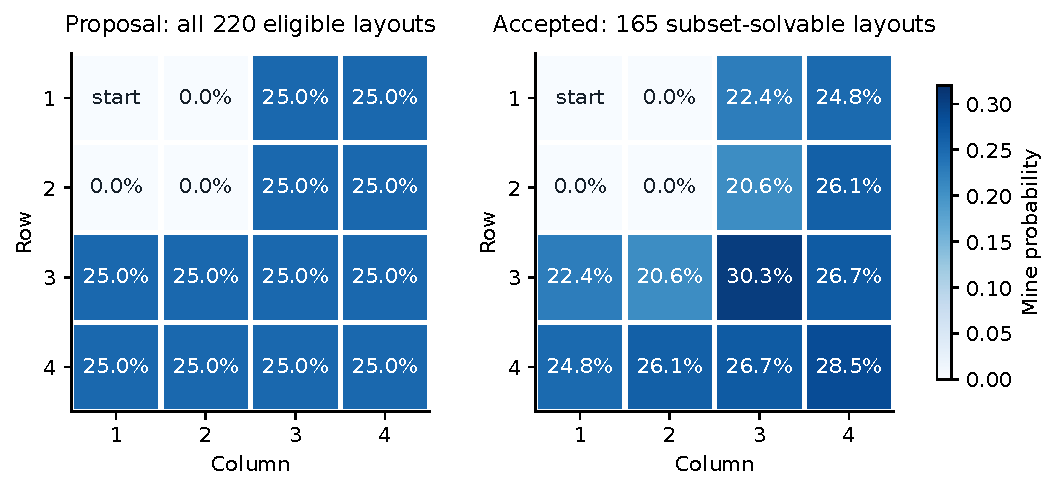
\includegraphics[width=.96\linewidth]{figures/marginals.pdf}
\caption{Exact mine marginals for a corner-zero start on the $4\times4$, three-mine board. The four protected cells remain mine-free. Subset-solvability changes probabilities elsewhere without changing the total number of mines.}
\label{fig:marginals}
\end{figure}

The tiny-board exceptions are visible in the same table. The corner-safe subset set contains its 165 zero-start layouts plus the single layout with all three neighboring cells mined. At the interior safe start, 52 of the 87 accepted layouts have a positive initial clue. Those exceptions do not contradict the standard-difficulty proposition, whose mine-count assumptions fail here. Likewise, ``interior is easier'' depends on the proposal: interior zero acceptance is 100\%, but interior safe acceptance is only 19.12\%, below the corner-safe rate. If corner and interior starts were proposed equally and resampled after every failure, the corner-safe share of accepted subset boards would be $166/(166+87)=65.61\%$, rather than 50\%.

For a separate Monte Carlo check, we use the corner-zero subset event, whose exact acceptance rate is $p=165/220=3/4$. A seeded SHA-256 counter stream supplies 32-bit words; integer rejection removes index-modulo bias \emph{under the uniform-word model}. We draw uniform indices into the complete proposal list until obtaining 10,000 accepted layouts. The observed mean proposal count is 1.3386, compared with $1/p=1.3333$. The largest absolute mine-marginal discrepancy is 0.00675, or 0.675 percentage points. A separate 10,000-run experiment capped at three proposals fails 162 times (1.620\%), compared with $(1/4)^3=1.5625\%$. Its mean executed count is 1.3252, compared with 1.3125 from \eqref{eq:cap}.

\begin{figure}[htbp]
\centering
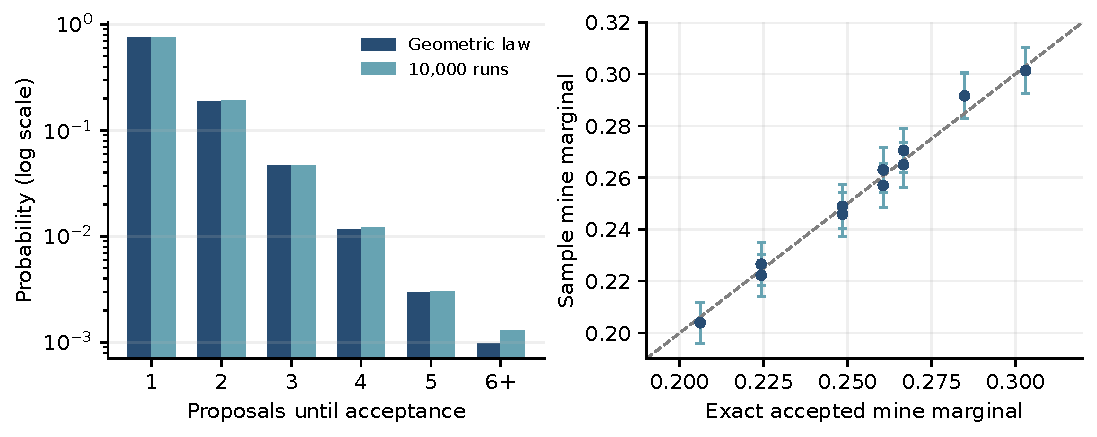
\includegraphics[width=.96\linewidth]{figures/sampling.pdf}
\caption{Rejection-sampling check against exact predictions. Left: proposal counts, with counts of six or more pooled. Right: eligible-cell mine marginals; vertical bars are individual normal-approximation 95\% intervals using exact Bernoulli variances and 10,000 outputs. They are not simultaneous intervals or a proof of the random generator's independence.}
\label{fig:sampling}
\end{figure}

\section{Posterior inference and implementation consequences}

If a player knows the generator law $Q$ and observes $O$, the correct layout posterior is
\begin{equation}
 \Prb_Q(L\mid O)=\frac{Q(L)\ind\{L\in\mathcal C(O)\}}{\sum_{L'\in\mathcal C(O)}Q(L')},\qquad
 \Prb_Q(i\in L\mid O)=\sum_{L\in\mathcal C(O)}\ind\{i\in L\}\Prb_Q(L\mid O).
 \label{eq:posterior}
\end{equation}
With ideal rejection from a uniform baseline, only accepted layouts consistent with $O$ remain equally likely. Ordinary clue-only probability calculation instead weights all baseline-consistent layouts. Those are different information models. An exact example in the accompanying data has 10 clue-consistent layouts after the initial corner opening, but only three compatible with the subset-NG generator. Cell $(4,1)$ has mine probability $1/2$ from clues alone and zero under that known generator. The stored layout mask is 8384 and visible mask 819, using zero-based row-major bit positions. Generator-aware inference should be claimed only when the sampler and its acceptance rule are actually known; an unspecified NG badge does not supply the required prior weights.

The local game's current NG control holds the upper-left start fixed, respects the selected safe-only or zero-opening proposal, and attempts at most 250 candidates. Certification uses the same bounded subset function inspected above. The engine uses seeded shuffling and derives candidate seeds from the base seed and attempt index. This makes runs reproducible, but it does not prove that proposals are independent or exactly uniform over all eligible layouts. In particular, a finite seed space cannot cover every layout on a large board with equal probability unless the support and multiplicities permit it. Equations~\eqref{eq:rejection}--\eqref{eq:cap} are exact for their declared ideal sampling assumptions; the finite enumeration is exact independently of those assumptions. The Monte Carlo stream is also deterministic pseudorandomness, used to check numerical agreement rather than establish a theorem about physical randomness.

A defensible NG generator therefore records its mine count, protected region, start, certifier version and bounds, proposal mechanism, rejection or repair method, and stopping policy. It returns only a certified board or an explicit failure. For a pure rejection design, stronger certification usually increases acceptance and changes the selected population. For a repair design, certification establishes playability while a separate analysis is needed for distribution. These distinctions explain both how NG games can remain unpredictable and why their spatial statistics can differ systematically from ordinary Minesweeper.

\paragraph{Reproducibility.}
Run \texttt{node enumerate.cjs} in this paper's folder, followed by \texttt{python3 figures.py} in an environment with NumPy and Matplotlib. The first command reads the local engine two directories above, saves its file and solver-function hashes, and writes \texttt{data/results.json}. That file contains exact accepted-layout masks, mine marginals, the uniqueness and stronger-solver examples, generator-aware posterior data, and the full sampling summaries. The second command creates the plotted PDF and PNG figures. Enumeration, direct deductions, exact inference, and rejection simulation are included in the source; only the subset certifier is imported from the game. All reported finite-population counts are checked for soundness and solver-set inclusion on this test board.

\begin{thebibliography}{9}
\small
\bibitem{tatham} Simon Tatham and contributors. \emph{Mines source}, as distributed in the Android Portable Puzzles source tree. Functions \texttt{minegen}, \texttt{minesolve}, and \texttt{mineperturb}. Inspected October 26, 2026. \url{https://github.com/chrisboyle/sgtpuzzles/blob/main/app/src/main/jni/mines.c}.
\bibitem{js-source} David N. Hill. \emph{JSMinesweeper: MinesweeperGame.js}. Function \texttt{createNoGuessGame}. Inspected October 26, 2026. \url{https://github.com/DavidNHill/JSMinesweeper/blob/master/Minesweeper/client/MinesweeperGame.js}.
\bibitem{js-doc} David N. Hill. \emph{JSMinesweeper documentation}. Player settings and replay behavior. Inspected October 26, 2026. \url{https://github.com/DavidNHill/JSMinesweeper}.
\bibitem{wom} Minesweeper Online. \emph{Gameplay: No guessing mode}. \url{https://minesweeper.online/help/gameplay}. Accessed October 26, 2026.
\end{thebibliography}
\end{document}
